\chapter{Macroblock Technique for Hybrid Solvers}
\label{chp:macroblocks}

In this chapter, we will explore an alternative approach for solving
elastic deformation problems. Compared to Chapter
\ref{chp:parallelization}, the approach outlined in this part of the
document will be focusing on the challenge of poor convergence when
using complex, non-linear materials. We will also be focusing on how
careful attention to the interplay between modern compute ability
verses memory availability can help us create more optimized solvers
for elastic materials. To do this, we will be targeting the common
approach used by many non-linear elastic simulations, namely the
combination of an outer Newton method around an inner linear solver.

The Newton method has largely been the golden standard for the
simulation of nonlinear elastic bodies, although a number of
interesting deviations from this standard approach have garnered
attention in the graphics literature (e.g., nonlinear multigrid cycles
~\citep{ZhuSTB:2010}, projective and position-based dynamics
~\citep{MuellHHR:2007,BouazMLKP:2014,Wang:2015} and shape matching
~\citep{RiverJ:2007}). In a typical Newton scheme, once a linear
approximation to the governing equations is computed, most
practitioners will either employ a direct method or select a technique
from a spectrum of iterative methods in order to solve the resulting
system.


\begin{figure}
 \begin{center} 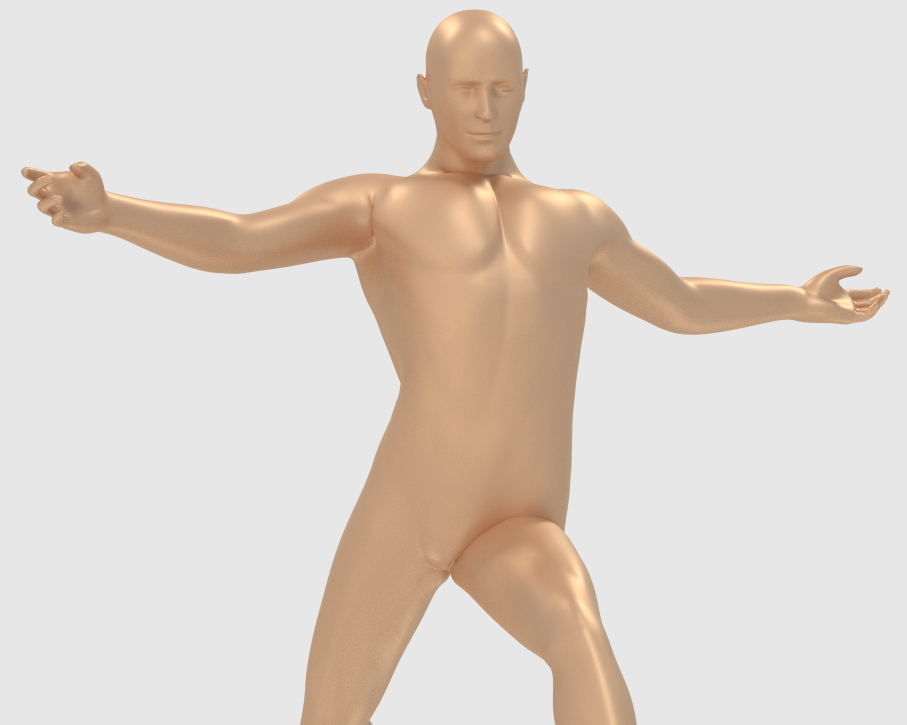
\includegraphics[width=.32\textwidth]{chapter_macroblocks/images/skinning_skin.png} 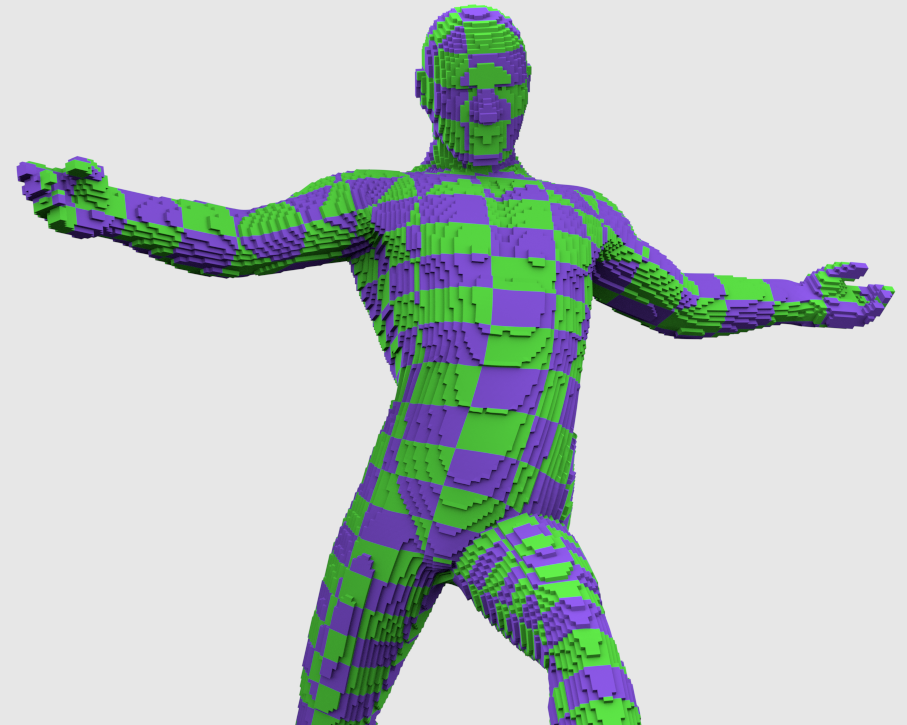
\includegraphics[width=.32\textwidth]{chapter_macroblocks/images/skinning_macroblocks.png} 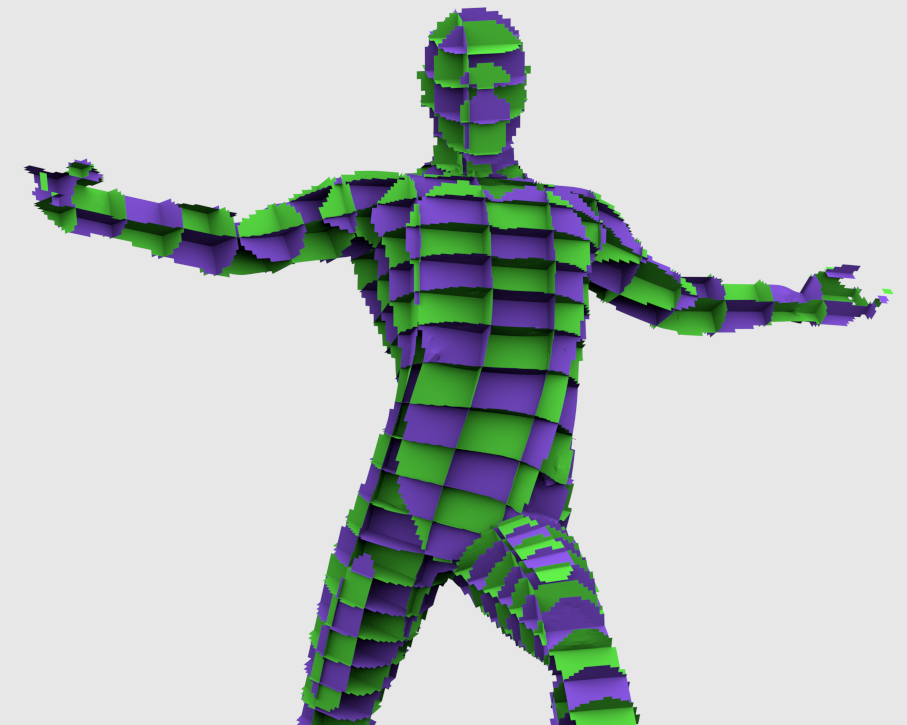
\includegraphics[width=.32\textwidth]{chapter_macroblocks/images/skinning_interface.png} \end{center}
 \caption{Deformed model alongside illustration of its constitutive
   macroblocks}{(Left) High resolution human mesh posed
   quasistatically by a skeleton with soft spring
   constraints. (Center) Embedding lattice divided into macroblocks
   (shown as alternating regions of green and purple). (Right)
   Illustration of the degrees of freedom along the macroblock
   boundaries. Conjugate Gradients is applied to a system with the
   size of these interface nodes. The model has 286K grid cells.}
 \label{fig:macroblocks:skinning-example}

 \end{figure} 

 Direct solvers are perhaps the safest and most straightforward way to
 solve the system that results from the linearization of the governing
 equations. These methods can be quite practical for relatively small
 problems when direct algebra is not very expensive. Additionally,
 these techniques are quite resilient to the conditioning of the
 underlying problem. Even for large models, high quality parallel
 implementations such as the Intel MKL PARDISO library are
 available. Despite such advantages, direct methods suffer from
 inherently superlinear computational complexity. Even with the
 benefit of parallelism, direct methods will typically be more
 expensive than several iterative schemes, especially if few number of
 iterations are performed. Additionally, direct methods are inherently
 memory bound; at the core of direct solvers are forward and backward
 substitution routines that carry out a very small number of
 arithmetic operations for each memory access required. This often
 results in grossly memory-bound execution profiles on modern
 hardware. This drawback is even more heavily felt for large models
 that do not fit in cache. Finally, each iteration of the Newton
 method is inherently inexact, providing only a step towards the
 converged solution. With direct methods we often find ourselves
 perfectly solving an inaccurate linearized approximation.

 With iterative solvers, we can aim for an approximate solution to the
 linearized problem with the understanding that with each Newton
 iteration the problem itself will change. These methods include
 Krylov methods like Conjugate Gradient, Multigrid, and fixed-point
 iterations such as Jacobi, Gauss-Seidel and SOR. The primary benefit
 of iterative techniques is that each individual iteration is
 relatively cheap; this allows users the option to either iterate as
 much as they can afford, or alternatively truncate the iterative
 process when the approximate solution is acceptable.  Also, many
 iterative methods are assembly-free, alleviating the need to
 construct or store the stiffness matrix.  In fact, some of the most
 efficient techniques go to great lengths to minimize memory footprint
 ~\citep{McAdaZSETTS:2011} while leveraging SIMD and multithreading.

 Iterative solvers often have to cope with challenges of their
 own. Local methods like Jacobi, GS, and SOR are slow to capture
 global effects, as they propagate information at a limited speed
 across the mesh. Krylov methods will typically prioritize the most
 important modes that contribute to a high residual; for example,
 consider a system with a few tangled elements that create large local
 forces.  Elements suffering from small errors will be relatively
 neglected by a method like Conjugate Gradients, while the solver
 focuses on the highly tangled elements before turning its attention
 to the bigger picture. Multigrid is an interesting alternative that
 often emerges as the performance champion; however, it can often be
 tricky to get to work robustly, and might be less appropriate for
 thin elastic objects, such as a thin flesh layer on a simulated
 face. Preconditioning can accelerate the convergence of iterative
 solvers but, in contrast to certain fluids simulation scenarios, the
 accelerated convergence might not always justify the increased
 per-iteration cost. Preconditioners based on incomplete
 factorizations are memory bound as they require matrix assembly, and
 generally require an expensive re-factorization step at each Newton
 iteration. We note that the same factorization overhead would be
 incurred even when the Newton method is nearly converged, where just
 a handful of iterations would suffice to solve the linearized
 equations. Multigrid-based preconditioners might achieve more
 competitive performance, but such approaches have been primarily
 tested in the area of fluid simulation ~\citep{FerstWD:2014} and not so
 much in nonlinear deformable solids.

 We propose a hybrid method that balances certain advantages of both
 direct and iterative schemes. Specifically we endeavor to achieve a
 good compromise between memory and compute load, reduce the memory
 footprint whenever possible, while significantly reducing iteration
 count. We pursue these goals while being competitive with the
 per-iteration cost of unpreconditioned CG. We employ a grid-based
 discretization, and aggregate rectangular clusters of cells into
 ``macroblocks'' with a proposed size of $16\times 8\times 8$ cells.
 These clusters essentially act as composite elements the same way
 that a typical hexahedral element can be thought of as a black box
 that takes displacements as inputs and produces nodal forces as
 output. However, our composite elements only take in displacements on
 the nodes of their periphery and return forces on those same boundary
 nodes. Using this construct we obtain an equivalent linear system
 with degrees of freedom only on cluster boundaries.

 \textbf{Scope} This chapter is an exploration of the performance
 potential offered by composite ``macroblock'' elements, initially
 focusing on the well-established simulation paradigm of a Newton-type
 scheme for solving a nonlinear system of governing equations. Thus,
 we only focus on grid-based discretizations of elasticity, and forgo
 the exploration of different simulation paradigms (e.g., multigrid,
 projective dynamics) where our formulation might still have a viable
 role.  Finally, we consciously restrict our investigation to
 grid-based models that do not exhibit non-local interactions, such as
 spring-based constraints or penalty-based self-collision resolution
 mechanisms (one-sided collisions between the elastic body and
 kinematic objects are supported).

%-------------------------------------------------------------------------


\begin{figure}
\begin{center}
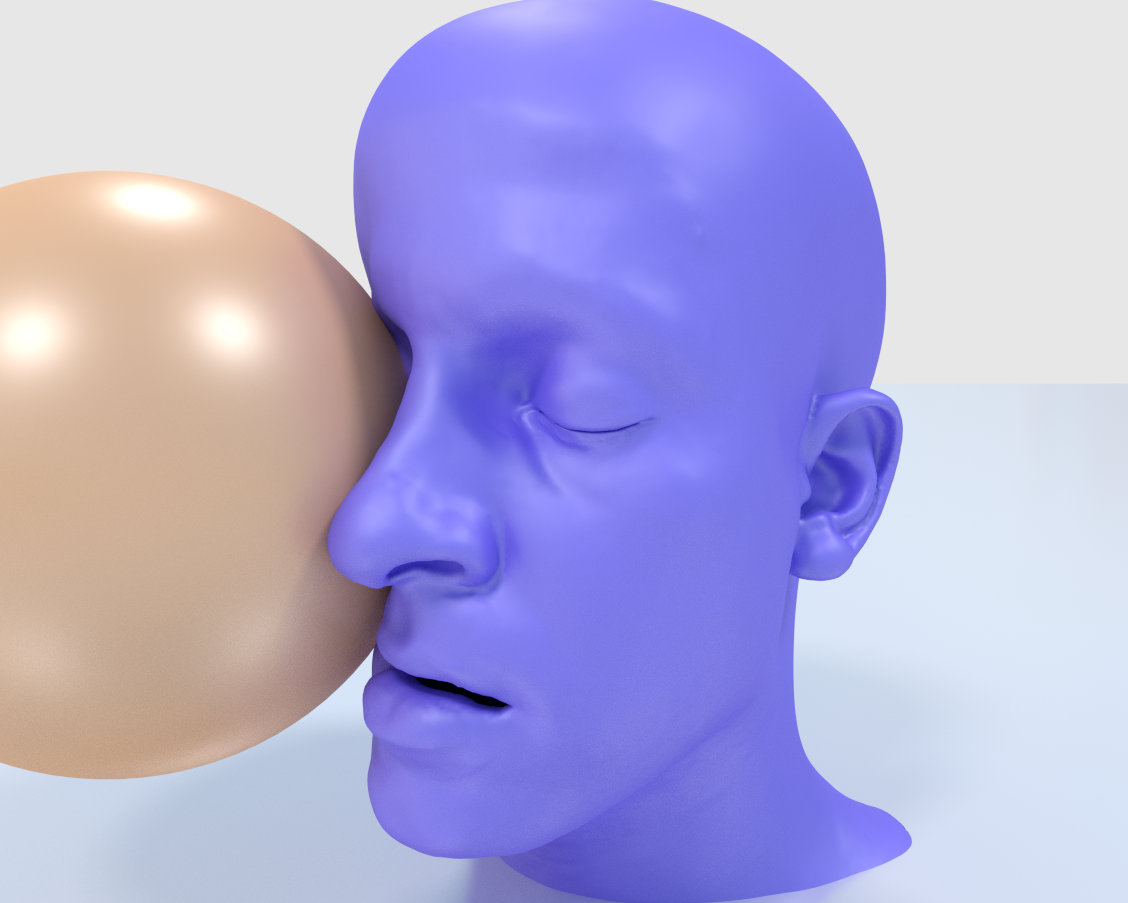
\includegraphics[width=.32\textwidth]{chapter_macroblocks/images/face_smash1.png}
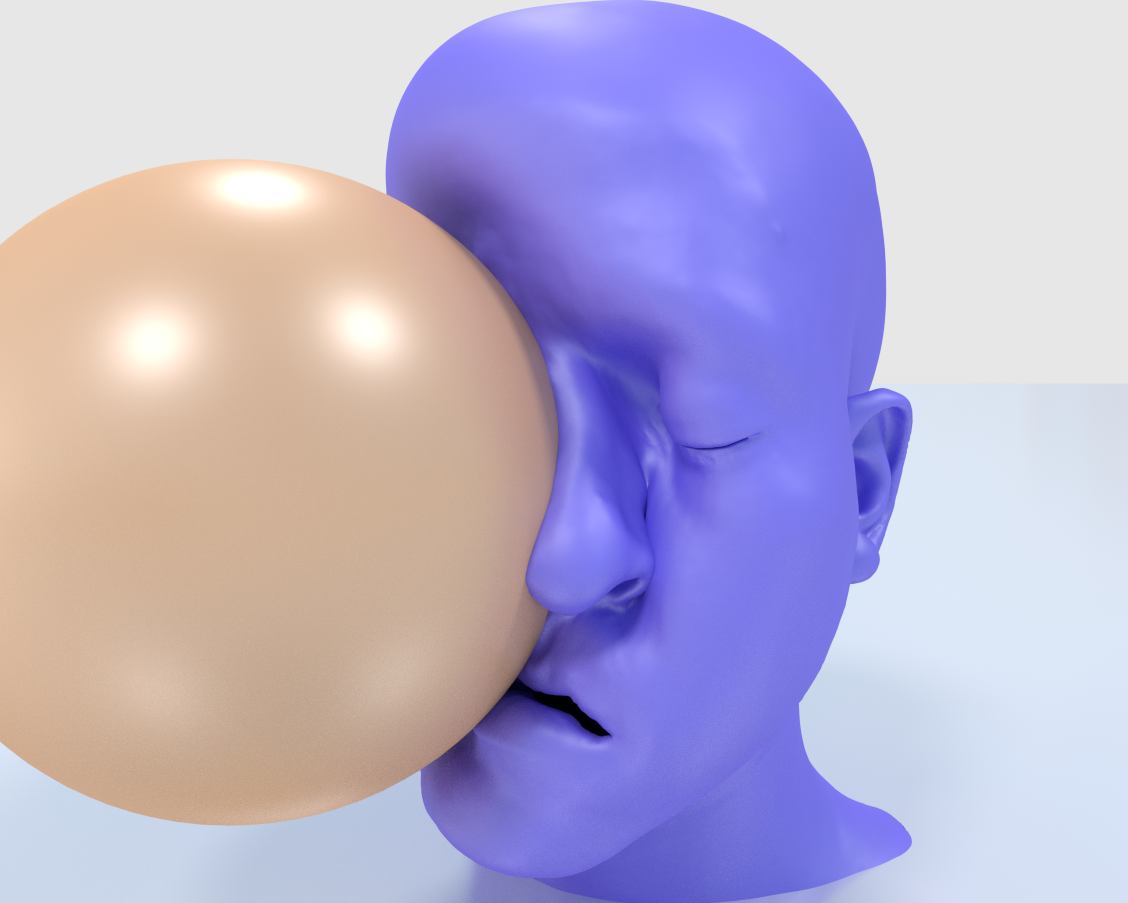
\includegraphics[width=.32\textwidth]{chapter_macroblocks/images/face_smash2.png}
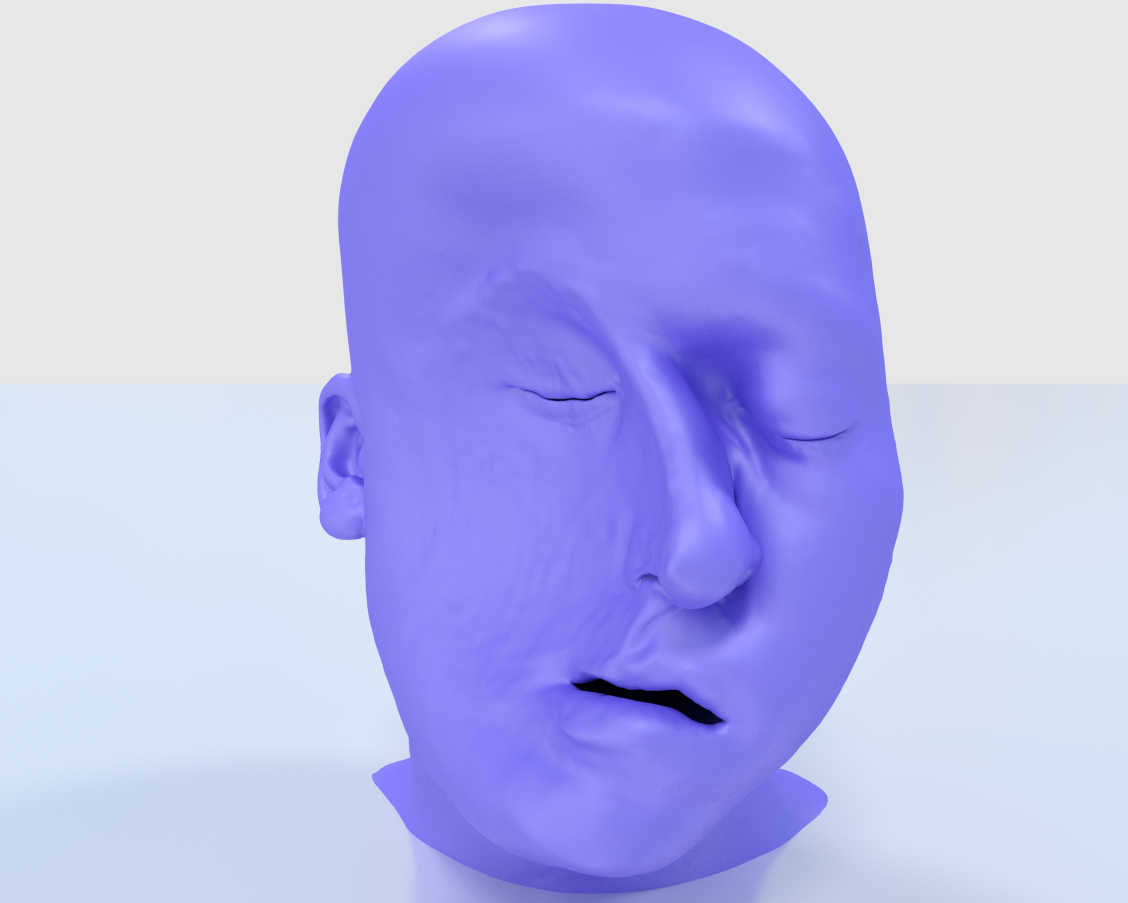
\includegraphics[width=.32\textwidth]{chapter_macroblocks/images/face_smash3.png} \end{center}

\caption{Macroblock solver used to handle rigid-elastic collision
  scenario }{A kinematic rigid sphere collides against a
  high-resolution embedded face model. The relatively small thickness
  of the elastic flesh, in addition to the topological features near
  the nose and mouth regions, would complicate the use of a typical
  multigrid solver ~\citep{McAdaZSETTS:2011} .}
 \label{fig:macroblocks:face-smash-example}
 \end{figure}

\section{Macroblock-based discretization and numerical solution}
\label{sec:macroblocks:discretization}

We start by reviewing the equations that our method targets, and
detailing how our proposed \emph{macroblock} concept can reformulate
them into an equivalent but more efficiently solvable form. This
process will necessitate the exact solution of several smaller systems
of equations, each in the order of a couple thousand of unknowns. In
this section we will simply assume that a highly efficient
\emph{direct} solver for those systems is available. Section
\ref{sec:macroblocks:local-solver} will provide the implementation details of this
highly optimized solver.

The governing equations describing the deformation of an elastic
nonlinear solid depend on the time integration scheme employed. For
example, in quasistatic simulation we have to solve the nonlinear
equilibrium equation $\mathbf{f}(\mathbf{x};t)=0$ at any time instance
$t$. Using an initial guess $\mathbf{x}_n$ of the solution,
Newton's method computes a correction
$\delta\mathbf{x}=\mathbf{x}_{n+1}\!\!-\!\mathbf{x}_n$ by
solving the linearized system:
\begin{equation}
  \bigg(
\underbrace{\left.
-\frac{\partial\mathbf{f}}{\partial\mathbf{x}}
\right|_{\mathbf{x}_n}
}_{\mathbf{K}(\mathbf{x}_n)}
\bigg) \ 
\delta\mathbf{x}=\mathbf{f}(\mathbf{x}_n)
\label{eqn:macroblocks:quasistatic}
\end{equation}
If an implicit Backward Euler scheme was used, a system with similar
structure would form the core of Newton's method ~\citep{SifakB:2012}:
\begin{equation}
\left[(1\!\!+\!\!\frac{\gamma}{\Delta t})\mathbf{K}(\mathbf{x}_n)\!+\!\frac{1}{\Delta t^2}\mathbf{M}\right]
\delta\mathbf{x}=\frac{1}{\Delta t}\mathbf{M}(\mathbf{v}_p\!\!-\!\mathbf{v}_n)+\mathbf{f}(\mathbf{x}_n,\mathbf{v}_n)
\label{eqn:macroblocks:be}
\end{equation}
where $\mathbf{M}$ is the mass matrix, $\gamma$ is the Rayleigh
coefficient, $\mathbf{v}_p$ the velocities at the previous time step,
and $\mathbf{f}$ now includes both elastic and damping forces (see
~\citep{SifakB:2012} for further details).

Despite the semantic differences, the linear systems in equations
(\ref{eqn:macroblocks:quasistatic}) and (\ref{eqn:macroblocks:be}) are very similar from an
algebraic standpoint:
\begin{itemize}
\item{Their coefficient matrices are both symmetric positive definite.}
\item{Their coefficient matrices have the same sparsity pattern.}
\item{In a grid-based discretization, their coefficient matrices can
    be assembled from the contributions of individual grid cells.}
\end{itemize}

We note that in order for this last property to hold true, we have
assumed that our elastic model does not have any interactions between
remote parts of its domain, such as penalty forces used to enforce
self-collision (which we consciously excluded from our
scope). Incidentally, penalty forces used to enforce collisions with
external kinematic bodies are allowed, since their point of
application on the elastic body can be embedded in a single grid
cell. For brevity, we will write any linear system that shares the
three properties above using the simplified notation $\mathbf{Kx=f}$,
without individual emphasis on whether the system originated from a
quasistatic, or a dynamic implicit scheme as in equations
(\ref{eqn:macroblocks:quasistatic}) and (\ref{eqn:macroblocks:be}), respectively.

The crucial next step in our proposed approach is a partitioning of
the active grid cells into \emph{macroblocks}, which are grid-aligned
rectangular clusters of a predetermined size, as illustrated in figure
\ref{fig:macroblocks:skinning-example}. In our implementation we use macroblocks
with dimensions of $16\times 8\times 8$ grid cells, although the
formulations in this section are largely independent of the macroblock
size. Section \ref{sec:macroblocks:analysis} provides the reasoning behind the
choice of this particular size of a macroblock.

Each macroblock $\mathcal{B}_i$ consists of up to
$16\times 8\times 8=1024$ grid cells $C_{i_1},C_{i_2},\ldots,C_{i_M}$;
note that in some cases this maximum number of constituent cells will
not be reached, if the macroblock overlaps with the boundary of the
elastic object, or if ``gaps'' of empty grid cells are present within
its extent. Similarly, up to $17\times 9\times 9$ nodal degrees of
freedom will be present in the region spanned by $\mathcal{B}_i$. Up
to $15\times 7\times 7$ of them will be on the \emph{interior} of
$\mathcal{B}_i$ and thus will not be touched by any other macroblock;
we will denote this interior node set with $I_i$. The remaining nodes,
located on the \emph{boundary} of $\mathcal{B}_i$ are potentially
shared by neighboring macroblocks; we will call these \emph{interface
  nodes} (as they reside at the interface between macroblocks) and
denote their set with $\Gamma_i$. All sets $I_i$ are clearly disjoint,
and we will denote their union by $\mathrm{I}=\cup I_i$. The interface
sets $\Gamma_i$ do overlap with one another, and we denote their union
by $\Gamma=\cup\Gamma_i$. For large enough models, we expect around
$72\%$ of grid nodes to lie in some interior set, and approximately
$28\%$ on the interface set $\Gamma$, using the aforementioned
macroblock size.

Our objective will be to replace the linear system $\mathbf{Kx=f}$
with an equivalent system, which only includes the interface nodes in
$\Gamma$ as unknowns. To do so, we first write the system in block
form, by separating interior and interface variables as follows:
$$
\left(
\begin{array}{cc}
\mathbf{K}_{\mathrm{I}\mathrm{I}} & \mathbf{K}_{\mathrm{I}\Gamma} \\
\mathbf{K}_{\Gamma \mathrm{I}} & \mathbf{K}_{\Gamma\Gamma}
\end{array}
\right)
\left(
\begin{array}{c}
\mathbf{x}_{\mathrm{I}} \\
\mathbf{x}_{\Gamma}
\end{array}
\right)
=
\left(
\begin{array}{c}
\mathbf{f}_{\mathrm{I}} \\
\mathbf{f}_{\Gamma}
\end{array}
\right)
$$
Using block Gauss elimination, this system can be converted to the
following equivalent block-triangular form:
\begin{equation}
\left(
\begin{array}{cc}
\!\!\mathbf{K}_{\mathrm{I}\mathrm{I}}\!\!\! & \!\!\!\mathbf{K}_{\mathrm{I}\Gamma}\!\! \\
\!\!\mathbf{0}\!\!\! & \!\!\!\mathbf{K}_{\Gamma\Gamma}- \mathbf{K}_{\Gamma\mathrm{I}}\mathbf{K}_{\mathrm{I}\mathrm{I}}^{-1}\mathbf{K}_{\mathrm{I}\Gamma}\!\!
\end{array}
\right)
\left(
\begin{array}{c}
\!\!\mathbf{x}_{\mathrm{I}}\!\! \\
\!\!\mathbf{x}_{\Gamma}\!\!
\end{array}
\right)
=
\left(
\begin{array}{c}
\!\!\mathbf{f}_{\mathrm{I}}\!\! \\
\!\!\mathbf{f}_{\Gamma}-\mathbf{K}_{\Gamma\mathrm{I}}\mathbf{K}_{\mathrm{I}\mathrm{I}}^{-1}\mathbf{f}_{\mathrm{I}}\!\!
\end{array}
\right)
\label{eqn:macroblocks:schur}
\end{equation}


\begin{figure}
\begin{center}
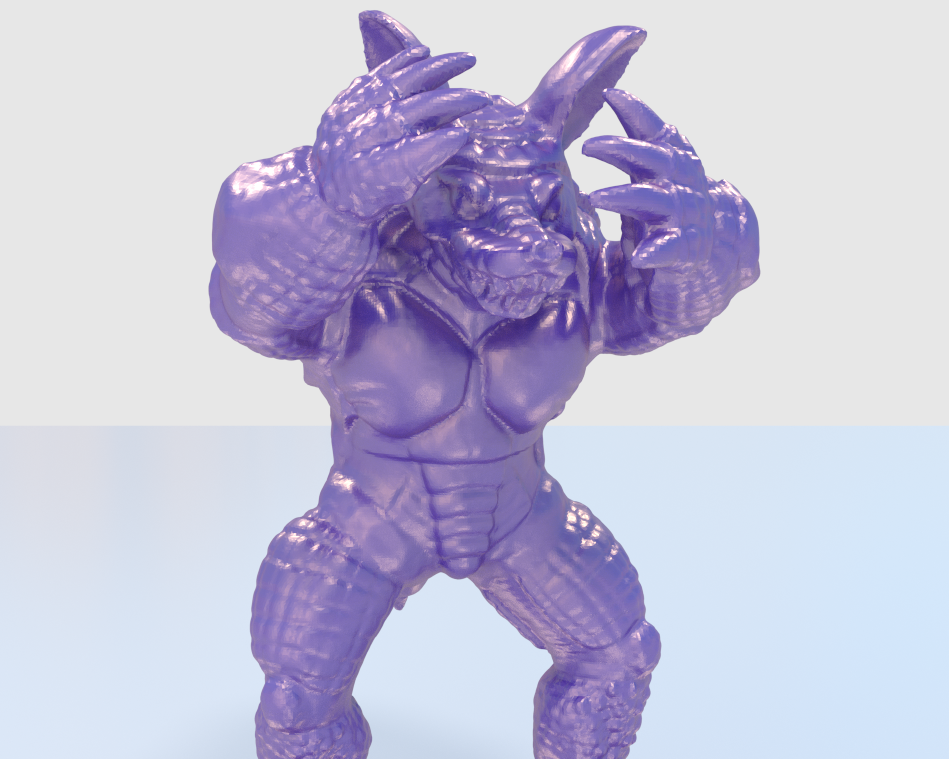
\includegraphics[width=.32\textwidth]{chapter_macroblocks/images/armadillo1.png}
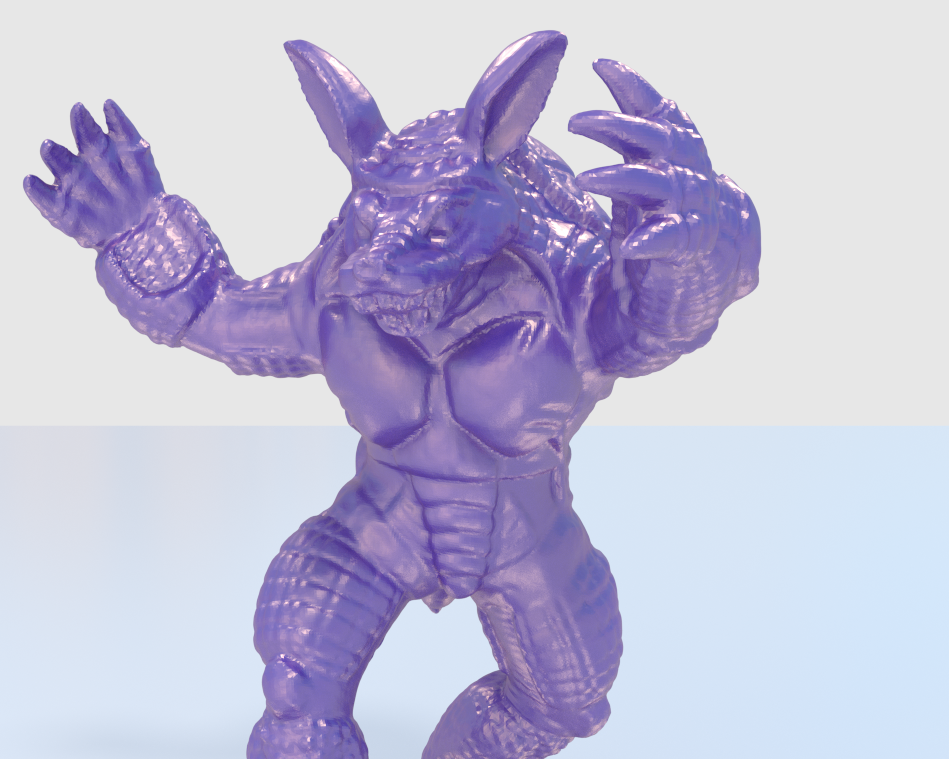
\includegraphics[width=.32\textwidth]{chapter_macroblocks/images/armadillo2.png}
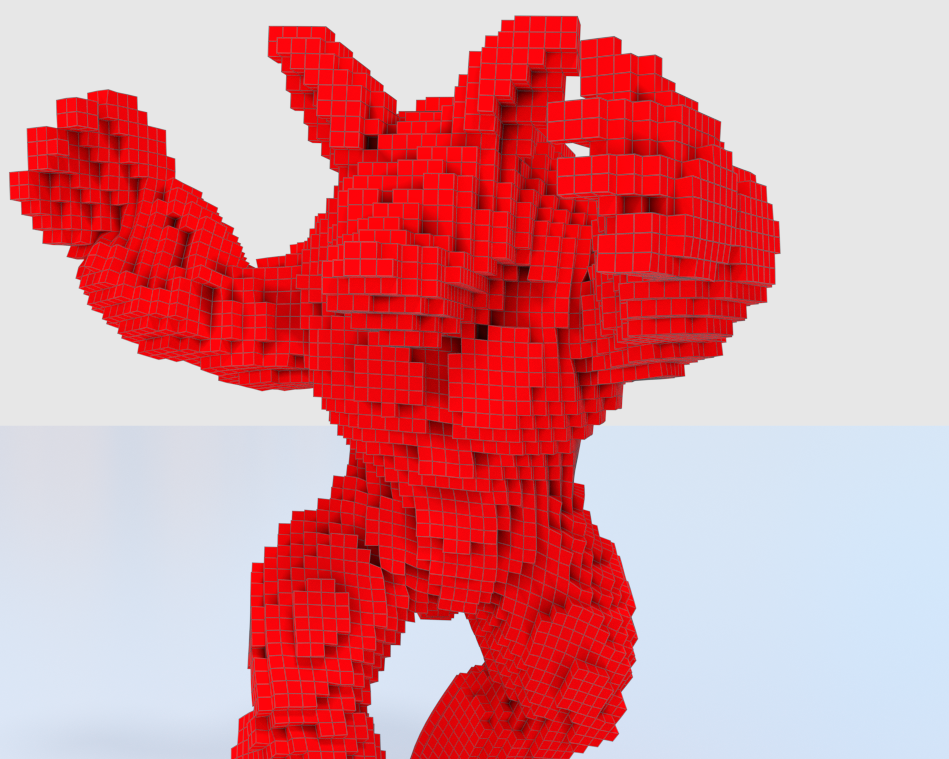
\includegraphics[width=.32\textwidth]{chapter_macroblocks/images/armadillo3.png}
\end{center}
\caption{Macroblock solver used to handle basic quasistatic pose
  scenario}{Armadillo model deforming as a result of kinematically
  animated Dirichlet constraints. Embedding lattice shown on the
  right.}
 \label{fig:macroblocks:armadillo-example}
\end{figure}

Equation (\ref{eqn:macroblocks:schur}) suggests the following algebraically
equivalent method for solving the system $\mathbf{Kx=f}$:

\noindent\textbf{Step 1} Compute an interface-specific right hand
side, from the bottom block of the right hand side of system
(\ref{eqn:macroblocks:schur}):
\begin{equation}
\hat{\mathbf{f}}_{\Gamma}=\mathbf{f}_{\Gamma}-\mathbf{K}_{\Gamma\mathrm{I}}\mathbf{K}_{\mathrm{I}\mathrm{I}}^{-1}\mathbf{f}_{\mathrm{I}}
\label{eqn:macroblocks:ItoGamma}
\end{equation}
\noindent\textbf{Step 2} Solve the interface-specific system $\hat{\mathbf{K}}\mathbf{x}_\Gamma=\hat{\mathbf{f}}_{\Gamma}$ to compute the values $\mathbf{x}_\Gamma$ of all
interface nodes. Note that the matrix of the system
\begin{equation}
\hat{\mathbf{K}}=\mathbf{K}_{\Gamma\Gamma}- \mathbf{K}_{\Gamma\mathrm{I}}\mathbf{K}_{\mathrm{I}\mathrm{I}}^{-1}\mathbf{K}_{\mathrm{I}\Gamma}
\label{eqn:macroblocks:KGamma}
\end{equation}
is the Schur complement of the symmetric positive definite original
matrix $\mathbf{K}$, hence it is symmetric and positive definite in
its own right. We will solve this system, which only involves
interface degrees of freedom, using Conjugate Gradients.

\noindent\textbf{Step 3} Conclude the computation by solving for the
interior nodal variables from the top block of system
(\ref{eqn:macroblocks:schur}) as:
\begin{equation}
\mathbf{x}_{\mathrm{I}}=\mathbf{K}_{\mathrm{I}\mathrm{I}}^{-1}\left(\mathbf{f}_{\mathrm{I}}-\mathbf{K}_{\mathrm{I}\Gamma}\mathbf{x}_{\Gamma}\right)
\label{eqn:macroblocks:GammatoI}
\end{equation}
In order to reproduce the exact solution of $\mathbf{Kx=f}$, we would
need to solve the interface problem
$\hat{\mathbf{K}}\mathbf{x}_\Gamma=\hat{\mathbf{f}}_{\Gamma}$ in Step
2 exactly. However, given that we only use this solution as part of an
iterative Newton update, there is nothing preventing us from stopping
the Conjugate Gradients solver for the interface system short of full
convergence. However, as we discuss in sections \ref{sec:macroblocks:examples} and
\ref{sec:macroblocks:cgcompare}, the interface problem requires far fewer CG
iterations to produce good quality results than the same Krylov method
applied to $\mathbf{Kx=f}$. Furthermore, the optimizations of the
following section allow us to make the per-iteration cost of CG on the
interface problem be comparable to each CG iteration on the original
problem, resulting in a significant net performance gain.  When
assessing the cost of Steps 1-3, it is important to observe the
following:

\noindent\textbf{Inversion of $\mathbf{K}_{\mathrm{I}\mathrm{I}}$ is the main performance challenge}. The most performance-sensitive component of this process is
the multiplication with the inverse
$\mathbf{K}_{\mathrm{I}\mathrm{I}}^{-1}$ of the matrix block
corresponding to variables interior to macroblocks. Nevertheless,
since there is no direct coupling (in $\mathbf{K}$) between interior
variables of neighboring macroblocks,
$\mathbf{K}_{\mathrm{I}\mathrm{I}}$ is a block diagonal matrix,
comprised of decoupled diagonal components for each set of interior
variables of each macroblock. We thus use multithreading to invert the
interior of each macroblock in a parallel and independent
fashion. Within each macroblock, we use the aggressively
SIMD-optimized \emph{direct} solver detailed in section
\ref{sec:macroblocks:local-solver} to perform the inversion exactly and
efficiently.

\noindent\textbf{Multiplication with $\mathbf{K}_{\mathrm{I}\Gamma},\mathbf{K}_{\Gamma\mathrm{I}}$ in Steps 1 \& 3 is inexpensive}. The off-diagonal blocks
$\mathbf{K}_{\mathrm{I}\Gamma}$ and $\mathbf{K}_{\Gamma\mathrm{I}}$
appearing in Steps 1 and 3 are small and sparse sub-blocks of
$\mathbf{K}$. In addition, they are only used in two matrix-vector
multiplications across Steps 1 and 3 for an entire Newton iteration
(we will address their role in Step 2, next). These matrices can be
efficiently stored in sparse format, and their multiplication with
vectors can be parallelized (in our implementation, via SIMD within
macroblocks and multithreading across blocks). These matrices have
minimal performance impact in our examples.


\noindent\textbf{Conjugate Gradients does not need to construct $\hat{\mathbf{K}}$}. The interface matrix $\hat{\mathbf{K}}$, being a Schur complement, is significantly denser than
the original matrix $\mathbf{K}$; for example, any two nodal variables
on the interface of the same macroblock would be coupled
together. Fortunately, the Conjugate Gradients method does not need
this matrix to be explicitly constructed. Instead, the only
requirement is to be able to compute matrix-vector products of the
form
$$
\mathbf{s}_\Gamma=\hat{\mathbf{K}}\mathbf{p}_\Gamma=\left(\mathbf{K}_{\Gamma\Gamma}- \mathbf{K}_{\Gamma\mathrm{I}}\mathbf{K}_{\mathrm{I}\mathrm{I}}^{-1}\mathbf{K}_{\mathrm{I}\Gamma}\right)\mathbf{p}_\Gamma
$$
for any given input vector $\mathbf{p}_\Gamma$. In fact, we can compute such products on a per-macroblock basis. We start by computing the restriction of
$\mathbf{p}_\Gamma$ to the boundary $\Gamma_i$ of each macroblock $\mathcal{B}_i$, which we denote by $\mathbf{p}_{\Gamma_i}$. Subsequently, we compute a partial contribution to
the matrix-vector product as
\begin{equation}
\mathbf{s}_{\Gamma_i}=\hat{\mathbf{K}}_i\mathbf{p}_{\Gamma_i}=\left(\mathbf{K}_{\Gamma_i\Gamma_i}-
  \mathbf{K}_{\Gamma_i\mathrm{I}_i}\mathbf{K}_{\mathrm{I}_i\mathrm{I}_i}^{-1}\mathbf{K}_{\mathrm{I}_i\Gamma_i}\right)\mathbf{p}_{\Gamma_i}
\label{eqn:macroblocks:one-block}
\end{equation}
The highly efficient evaluation of the expression in equation
(\ref{eqn:macroblocks:one-block}) is precisely the focus of section
\ref{sec:macroblocks:local-solver}. We compute the contributions of all
macroblocks $\mathbf{s}_{\Gamma_i}$ in parallel, via multithreading,
and reduce them all together in a final summation to produce the
global result $\mathbf{s}_\Gamma$.

Finally, we point out a significant intuition behind the nature of the
macroblock-local Schur complement $\hat{\mathbf{K}}_i$, defined via
equation (\ref{eqn:macroblocks:one-block}). Similar to how an elemental stiffness
matrix maps nodal displacements to nodal force differentials for a
tetrahedral or hexahedral element, the \emph{macroblock stiffness
  matrix} $\hat{\mathbf{K}}_i$ directly maps displacements on the
boundary to forces on the same boundary nodes, under the assumption
that all interior nodes are functionally constrained to their exact
solution subject to the boundary displacement values. We note the
similarity of this concept to the work of \citet{GaoMS:2014},
although they used a Schur complement to abstract away the interior
nodes of an entire model, rather than assembling an elastic solid from
macroscopic cell blocks.


%-------------------------------------------------------------------------
\begin{figure}
\centering
\subfloat{%
  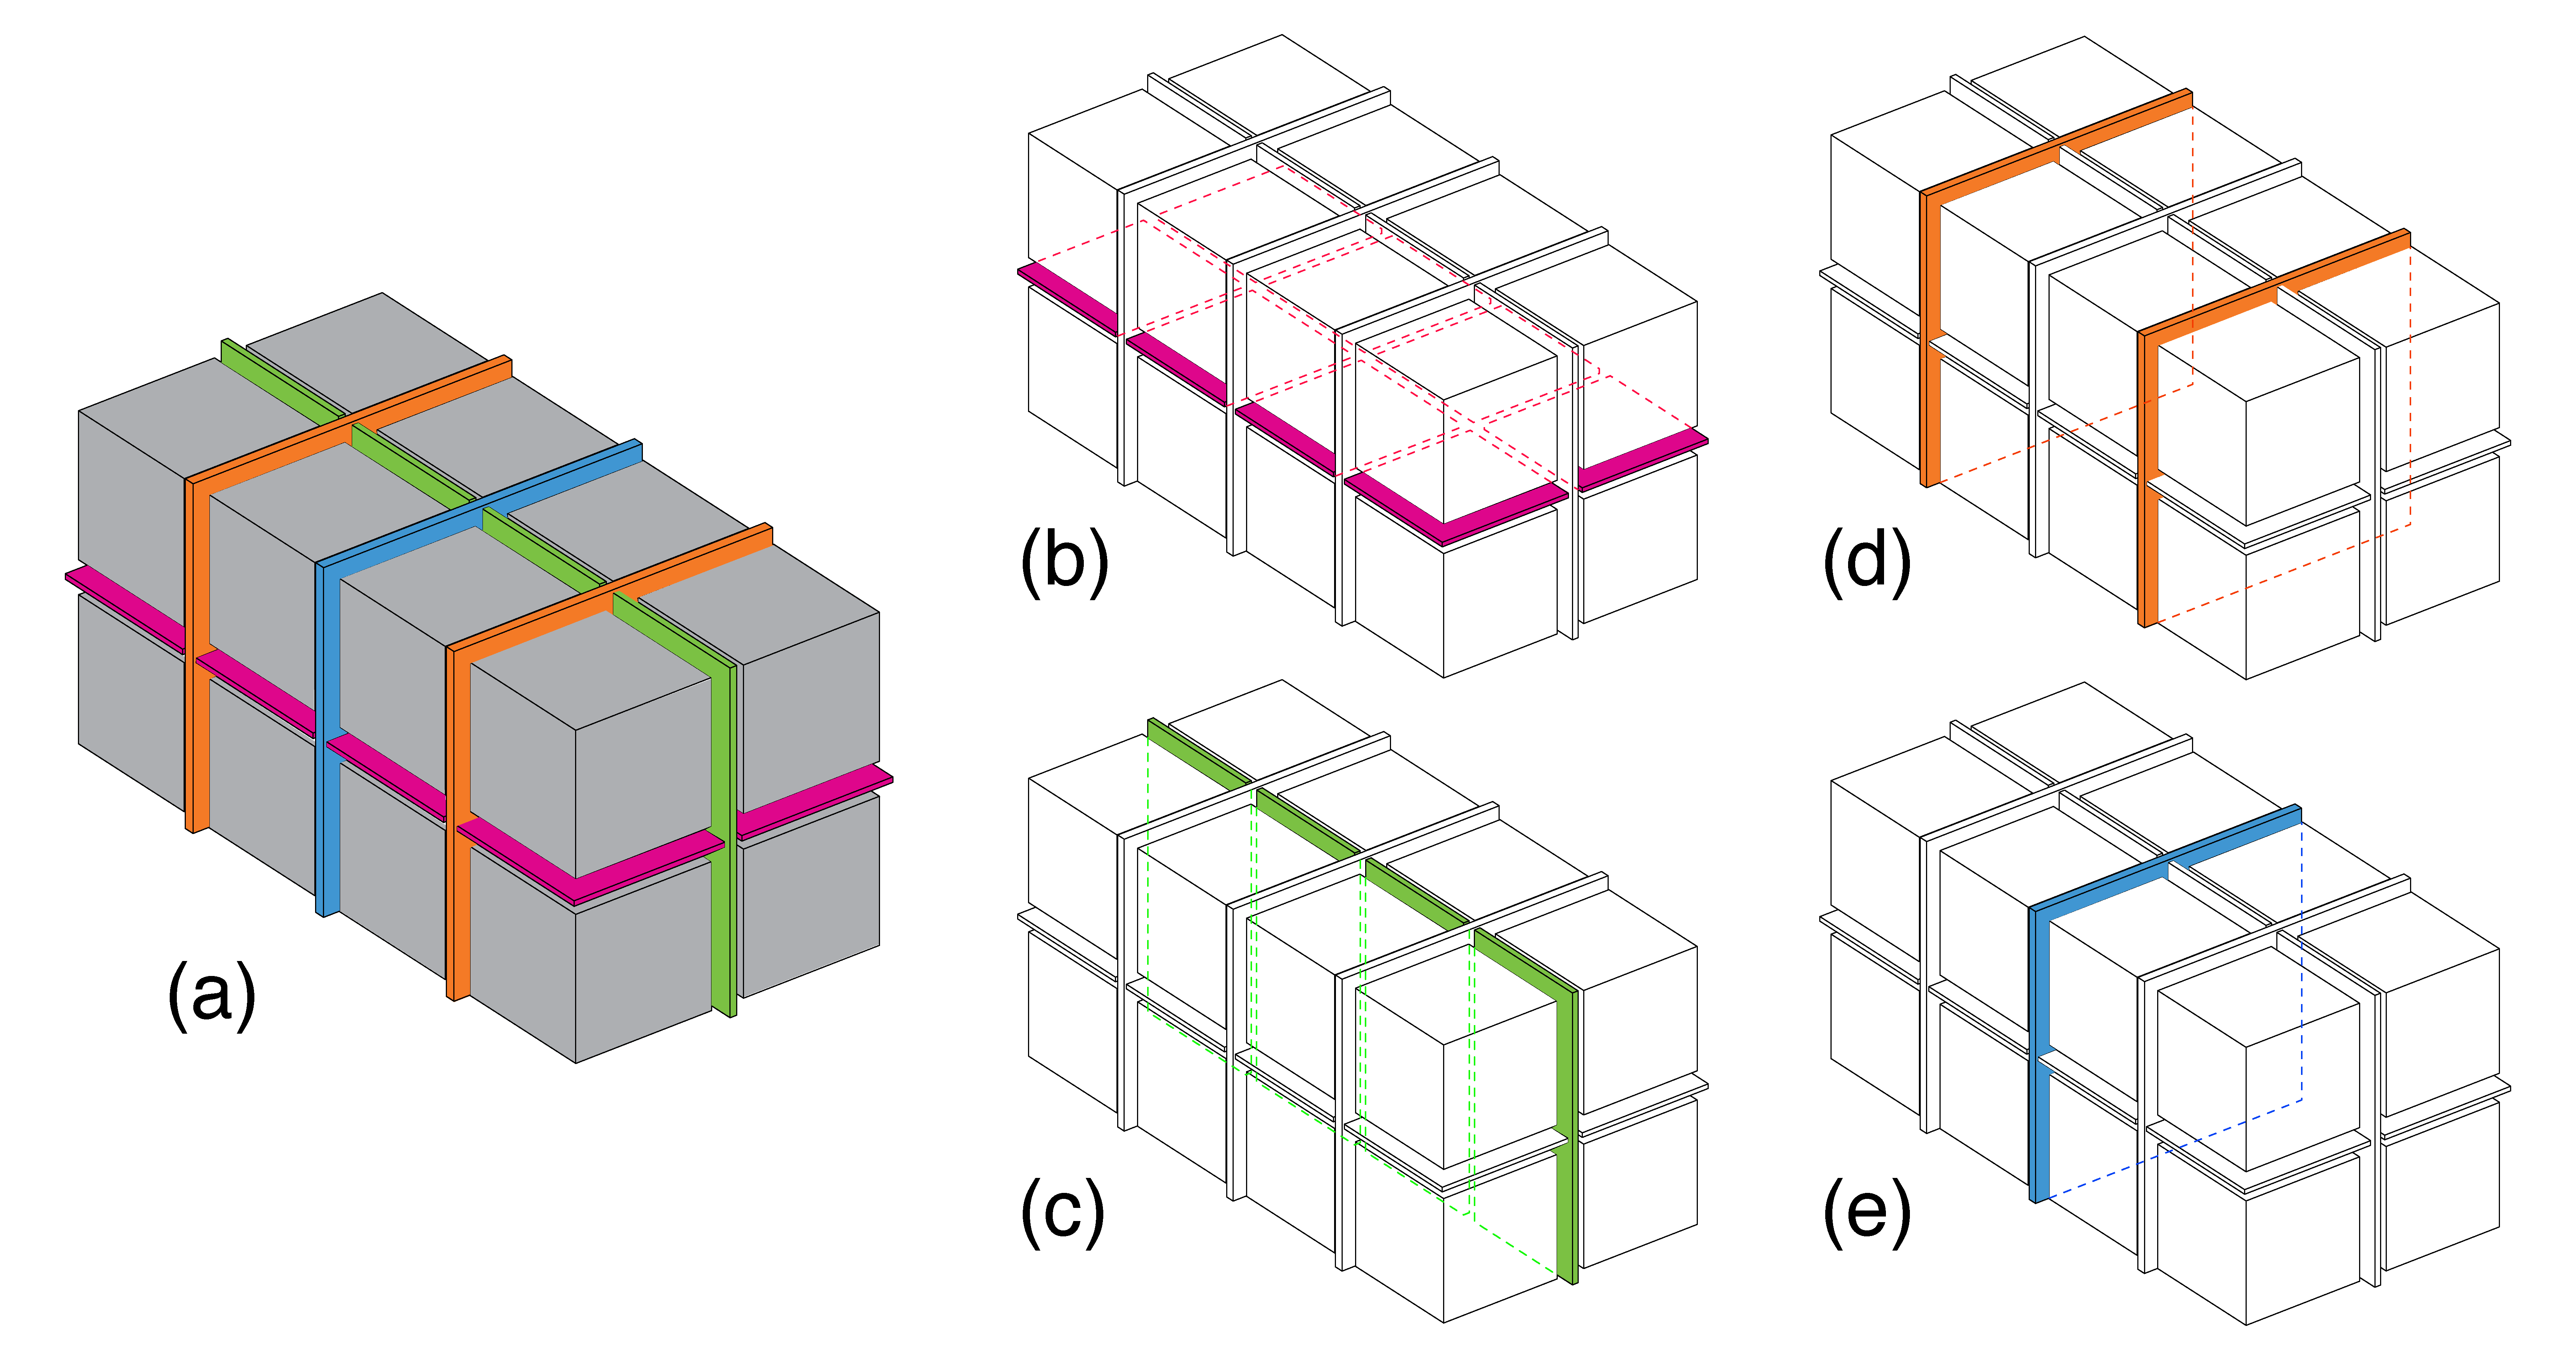
\includegraphics[height=2.2in]{chapter_macroblocks/images/macroblock_figure.pdf}
}

\subfloat{%
  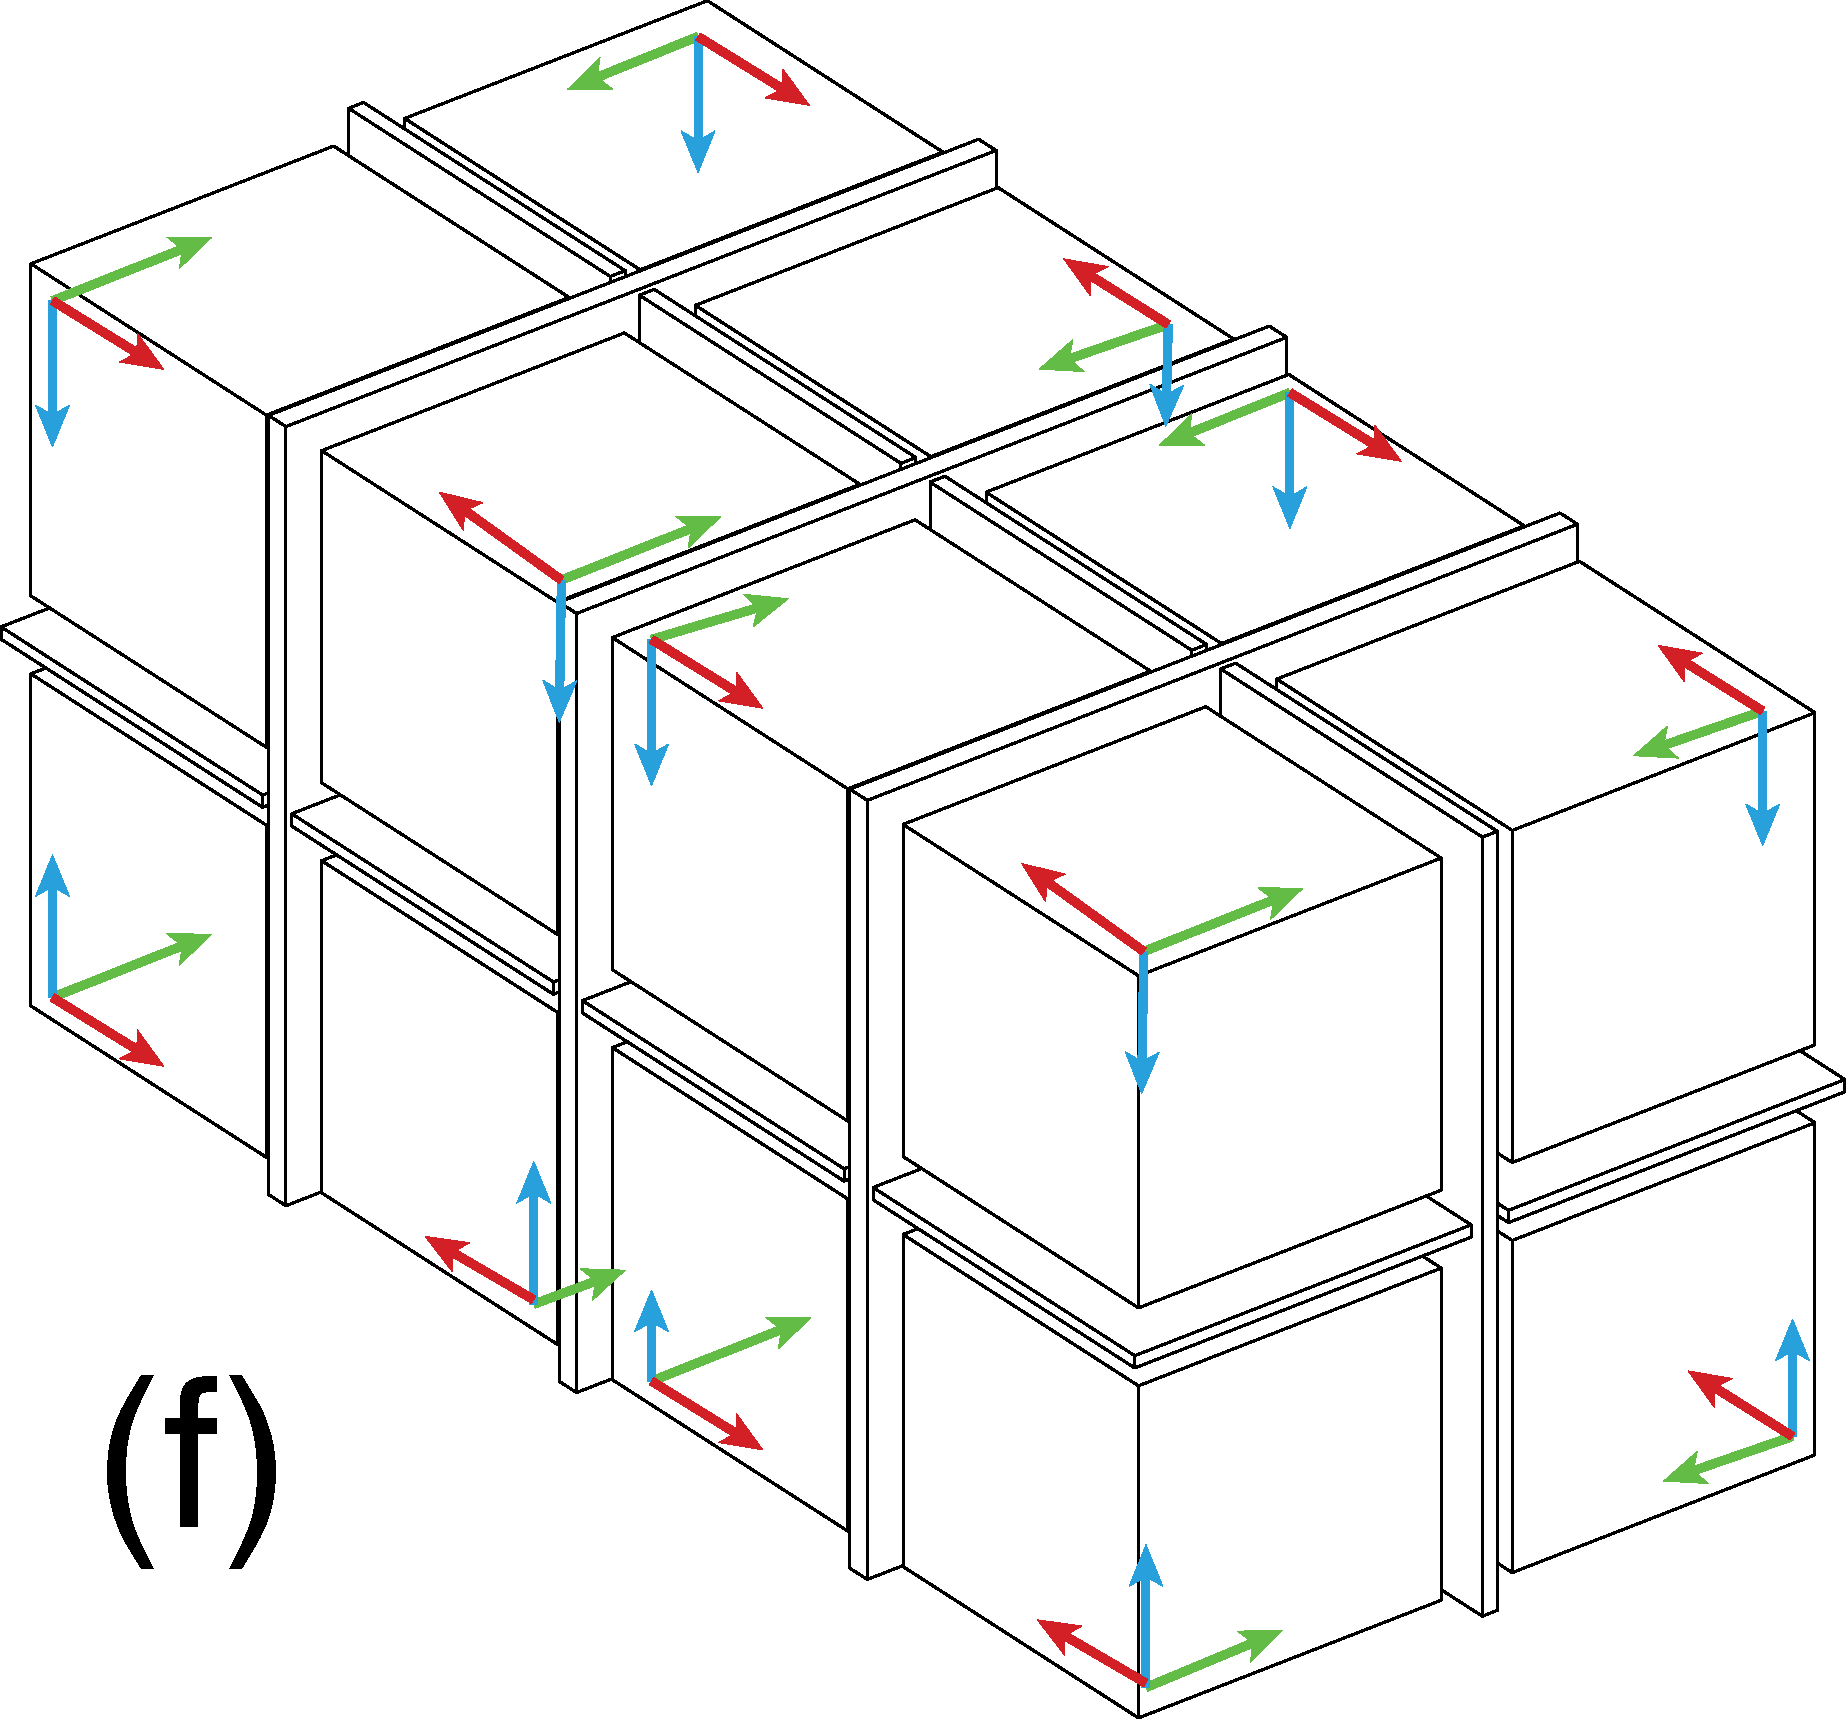
\includegraphics[height=2.2in]{chapter_macroblocks/images/macroblock_mirroring_figure.pdf}
}

\caption{Illustration of the internal macroblock divisions and
  structure}{The $15\!\times\!7\!\times\!7$ macroblock interior nodes
  are hierarchically subdivided, yielding (a) sixteen
  $3\!\times\!3\!\times\!3$ ``subdomains'' and (b,c,d,e) four
  ``interface'' layers. The first subdomain is reordered to maximize
  sparsity, and this ordering is mirrored (f) to the other 15
  subdomains.}
\label{fig:macroblocks:structure}


\end{figure}

\section{An optimized direct solver for macroblocks}
\label{sec:macroblocks:local-solver}

As outlined in section \ref{sec:macroblocks:discretization}, inverting
$\mathbf{K}_{\mathrm{I}_i\mathrm{I}_i}$ within each macroblock is the
most performance-sensitive part of our numerical approach. In this
section we explain how this operation can be performed with high
efficiency, by reducing its memory footprint and aggressively
leveraging instruction-level (SIMD) parallelism. We have designed a
numerical data structure containing the appropriate metadata and
computational routines to compute the matrix-vector product
$\mathbf{s}_{\Gamma_i}$ of equation (\ref{eqn:macroblocks:one-block}), given the
boundary values $\mathbf{p}_{\Gamma_i}$ as input. This structure
stores matrices $\mathbf{K}_{\Gamma_i\Gamma_i}$,
$\mathbf{K}_{\Gamma_i\mathrm{I}_i}$ and
$\mathbf{K}_{\mathrm{I}_i\Gamma_i}$ explicitly in compressed sparse
format (with slight modifications to facilitate SIMD parallelism, as
explained in section \ref{sec:macroblocks:vectorization}), as those are relatively
compact and inexpensive to multiply with. In addition, we store just
enough information to be able to multiply the interior inverse
$\mathbf{K}_{\mathrm{I}_i\mathrm{I}_i}^{-1}$ with input vectors,
without storing this matrix explicitly. As this section focuses on a
single macroblock $\mathcal{B}_i$, we omit the macroblock index $i$,
using the symbols $\mathrm{I}$ and $\Gamma$ to denote its interior and
interface nodes.

Given the sparsity and definiteness of
$\mathbf{K}_{\mathrm{I}\mathrm{I}}$, one straightforward approach
would be to compute its (exact) Cholesky factorization, under a
sparsity optimizing variable reordering. This factorization would take
place once per Newton iteration, while forward and backward
substitution passes would be used to apply the inverse in every
subsequent CG iteration based on equation (\ref{eqn:macroblocks:one-block}). We
do, in fact, compute exactly such a reordered Cholesky factorization;
however, instead of forward/backward substitution, we leverage a
hierarchical alternative (derived from the coefficients of the
computed factorization) that achieves the same result in significantly
less time, by reducing the required memory footprint.
%We start by describing the specific reordering we employ, and continue to explain our hierarchical solution process and SIMD vectorization steps. 

\subsection{Reordering}

We utilize a custom reordering of the $15\times 7\times 7$ interior
nodes of the macroblock, in order to optimize the sparsity of Cholesky
factorization and expose repetitive regular patterns that can be
matched with SIMD calculations. We define this reordering by means of
a hierarchical subdivision, as illustrated in figure
\ref{fig:macroblocks:structure}. First, we subdivide the $15\times 7\times 7$
interior region into two $7\times 7\times 7$ subregions, separated by
a $1\times 7\times 7$ interface layer, illustrated in blue color in
figure \ref{fig:macroblocks:structure}(e).  Each of these two regions is further
subdivided into two $3\times 7\times 7$ parts, separated by
$1\times 7\times 7$ interface layers, shown in orange in figure
\ref{fig:macroblocks:structure}(d).  Those $3\times 7\times 7$ regions are then
split into two $3\times 3\times 7$ parts, separated by
$3\times 1\times 7$ interfaces, shown in green in figure
\ref{fig:macroblocks:structure}(c).  A last subdivision results in two
$3\times 3\times 3$ subdomains, on either side of a
$3\times 3\times 1$ connector, drawn in magenta in figure
\ref{fig:macroblocks:structure}(b).  We refer to the resulting $3\times 3\times 3$
blocks as \emph{subdomains}, and the connective regions in figures
\ref{fig:macroblocks:structure}(b) through \ref{fig:macroblocks:structure}(e) as Level-1
through Level-4 \emph{interfaces}. We then proceed to compute a
minimum-degree reordering for one of the 16 resulting
$3\times 3\times 3$ subdomains, and \emph{mirror} this reordering
across their hierarchical interfaces to enumerate the nodes of all
remaining subdomains. This mirroring is essential in creating
repetitive patterns in the Cholesky factors, on which SIMD
optimizations are crucially dependent.  The final overall reordering
is formed by assembling a tree of this hierarchical subdivision (with
interfaces on parent nodes, and the regions they separate as their
children), and computing a reverse breadth-first tree traversal.

We have found this reordering to be optimal; it matches or outperforms
any heuristics (e.g., minimum-degree reordering in \textsf{Matlab}) in
the sparsity of the Cholesky factors. The resulting sparsity pattern
is illustrated in figure \ref{fig:macroblocks:sparsity}. Matrix
entries colored red are a subset (but not all) of the entries that
were filled-in during the Cholesky process. As expected, forward and
backward substitution on this matrix is a pronouncedly memory-bound
operation; hence we propose a further algorithmic modification that
produces the same result with approximately one-seventh of the memory
footprint. This alternative approach will only need to store the
number of coefficients corresponding to the \emph{black-colored}
entries in figure \ref{fig:macroblocks:sparsity}. The metadata for
this alternative approach, detailed next, will be harvested from the
Cholesky factorization just computed.

\subsection{Hierarchical factorization}

Consider the first hierarchical subdivision, illustrated in
\ref{fig:macroblocks:structure}(e), which separated the $15\times 7\times 7$ block
of interior nodes into two $7\times 7\times 7$ subregions, which we
denote by $\textrm{I}_1$ and $\textrm{I}_2$, along with a
$7\times 7\times 1$ connective region, denoted $\textrm{I}_c$ (drawn
blue in the figure above). If we reorder the matrix
$\mathbf{K}_{\textrm{II}}$ to expose this partitioning, it assumes the
following block form:
$$
\left(
\begin{array}{ccc}
\mathbf{K}_{11} & & \mathbf{K}_{1c} \\
& \mathbf{K}_{22} & \mathbf{K}_{2c} \\
\mathbf{K}_{c1} & \mathbf{K}_{c2} & \mathbf{K}_{cc}
\end{array}
\right)
$$
It can be easily verified that the \emph{inverse} of this matrix can
be written in the following Block-LDL form:
$$
\hspace*{-.15in}\left(
\begin{array}{ccc}
\!\!\!\mathbf{I}\!\!\!  & & -\mathbf{K}_{11}^{-1}\mathbf{K}_{1c}\!\!\! \\
& \!\!\!\mathbf{I}\!\!\! & -\mathbf{K}_{22}^{-1}\mathbf{K}_{2c}\!\!\! \\
& & \mathbf{I}\!\!\!
\end{array}
\right)\!\!
\left(
\begin{array}{ccc}
\!\!\!\!\mathbf{K}_{11}^{-1}\!\!\!\!\!  & &  \\
& \!\!\!\!\!\mathbf{K}_{22}^{-1}\!\!\!\!\! & \\
& & \!\!\!\!\!\mathbf{C}^{-1}\!\!\!\!
\end{array}
\right)\!\!
\left(
\begin{array}{ccc}
\!\!\!\mathbf{I}\!\!  & &  \\
& \mathbf{I} & \\
\!\!\!-\mathbf{K}_{c1}\mathbf{K}_{11}^{-1}\!\! & \!\!\!-\mathbf{K}_{c2}\mathbf{K}_{22}^{-1} & \!\!\!\mathbf{I}\!\!\!
\end{array}
\right)
$$
where
$\mathbf{C}=\mathbf{K}_{cc}-\mathbf{K}_{c1}\mathbf{K}_{11}^{-1}\mathbf{K}_{1c}-\mathbf{K}_{c2}\mathbf{K}_{22}^{-1}\mathbf{K}_{2c}$
is the Schur complement of $\mathbf{K}_{cc}$. With this formulation,
solving a problem
$\mathbf{K}_{\textrm{II}}\mathbf{x}_\textrm{I}=\mathbf{f}_\textrm{I}$
is equivalent to multiplying with the factorized version of
$\mathbf{K}_{\textrm{II}}^{-1}$ in the equation above. We make the
following significant observations:
\begin{itemize}
\item Other than the (seemingly elusive) inverses
  $\mathbf{K}_{11}^{-1},\mathbf{K}_{22}^{-1}$ and $\mathbf{C}^{-1}$,
  the factorization above does not incur any fill-in; factors such as
  $\mathbf{K}_{1c}$, etc. have the original sparsity found in
  sub-blocks of $\mathbf{K}_{\textrm{II}}$.
\item We can prove that the lower-triangular Cholesky factor of the
  Schur complement $\mathbf{C}$ is \emph{exactly} the bottom-rightmost
  (dense) diagonal block of the matrix shown in figure
  \ref{fig:macroblocks:sparsity} (also more prominently colored blue in figure
  \ref{fig:macroblocks:sparsity2}). Thus, multiplication with $\mathbf{C}^{-1}$
  can be performed simply via forward and backward substitution.
\item The inverses of the two subregions, $\mathbf{K}_{11}^{-1}$ and
  $\mathbf{K}_{22}^{-1}$ can be applied recursively using the exact
  same decomposition and block-LDL factorization described here, by
  splitting each $7\times 7\times 7$ into two $7\times 7\times 3$
  subregions and a $7\times 7\times 1$ connector as before. This
  recurrence can be unfolded until we arrive at the (sixteen)
  $3\times 3\times 3$ subdomains shown in figure
  \ref{fig:macroblocks:structure}. The Cholesky factors of those sixteen blocks
  are exactly the top-sixteen (sparse) diagonal blocks on the top-left
  of the Cholesky factorization in figure \ref{fig:macroblocks:sparsity}; thus
  those submatrices can be readily inverted without recursion.
\end{itemize}

\begin{figure}[h]

\centering{\includegraphics[width=.90\columnwidth]{chapter_macroblocks/images/Post_Extend_Sparsity.pdf}}

\caption{Illustration of macroblock sparsity patterns}{Sparsity of
  Cholesky factorization (with our optimal reordering), shown with red
  \textbf{and} black colors. The memory footprint of our proposed
  solver only includes the black-colored coefficients.}
\label{fig:macroblocks:sparsity}
\end{figure}

We note that the Cholesky factors of the Schur complement matrices
($\mathbf{C}$) that appear in deeper levels of this hierarchical
solution scheme are similarly harvested from the (dense) diagonal
blocks of the overall Cholesky factorization (highlighted in purple,
green and orange color in figure \ref{fig:macroblocks:sparsity2}, immediately
above the blue block at the bottom-rightmost part which corresponds to
the first hierarchical subdivision). At the final level of this
hierarchical solution process, we need the inverses of the matrix
blocks corresponding to the sixteen $3\times 3\times 3$ subdomains
themselves. For those blocks, we employ directly their sparse Cholesky
factorization, as seen in the top-sixteen (dark blue colored) diagonal
blocks in figure \ref{fig:macroblocks:sparsity2}, and solve using standard forward
and backward substitution.

It would appear that the additional computation that this recursive
solution entails would render it prohibitively expensive. However, the
stock Cholesky forward and backward substitution are memory-bound by
such a wide margin that our optimized recursive solution can afford to
execute a significantly larger amount of arithmetic operations, while
still being (barely, this time) bound by the time required to stream
the requisite matrix coefficients from memory into cache. The not so
obvious, but very significant, benefit is that the entire working set
of this solver is less than 800KB per macroblock, allowing all
subsequent memory accesses to occur exclusively in cache for every CPU
core handling an individual macroblock. Note that, although the
original reordered Cholesky factorization produces additional fill-in
on the matrix entries colored red in figure \ref{fig:macroblocks:sparsity}, our
recursive substitution process only touches a significantly sparser
subset of entries (colored black), requiring about 27\% of the entries
and 15\% of the storage footprint of the full, filled-in Cholesky
(accounting for row/column indices of structurally sparse blocks). In
section \ref{sec:macroblocks:examples} we provide the effective memory bandwidth
achieved by our macroblock solver, averaging between 13-18GB/s on a
10-core Haswell-EP Xeon processor.

\begin{figure}[h]

\centering{\includegraphics[width=.96\columnwidth]{chapter_macroblocks/images/Solver_Matrix_Components_Colored.pdf}}

\caption{Illustration of SIMD-instruction groupings of a macroblock
  matrix}{Our method reveals regular structures in the matrix sparsity
  pattern, exploiting them for vectorization. Same-color entries in
  the off-diagonal blocks can be processed with SIMD instructions.}
\label{fig:macroblocks:sparsity2}
\end{figure}

 \begin{figure*}[t!] \begin{center} 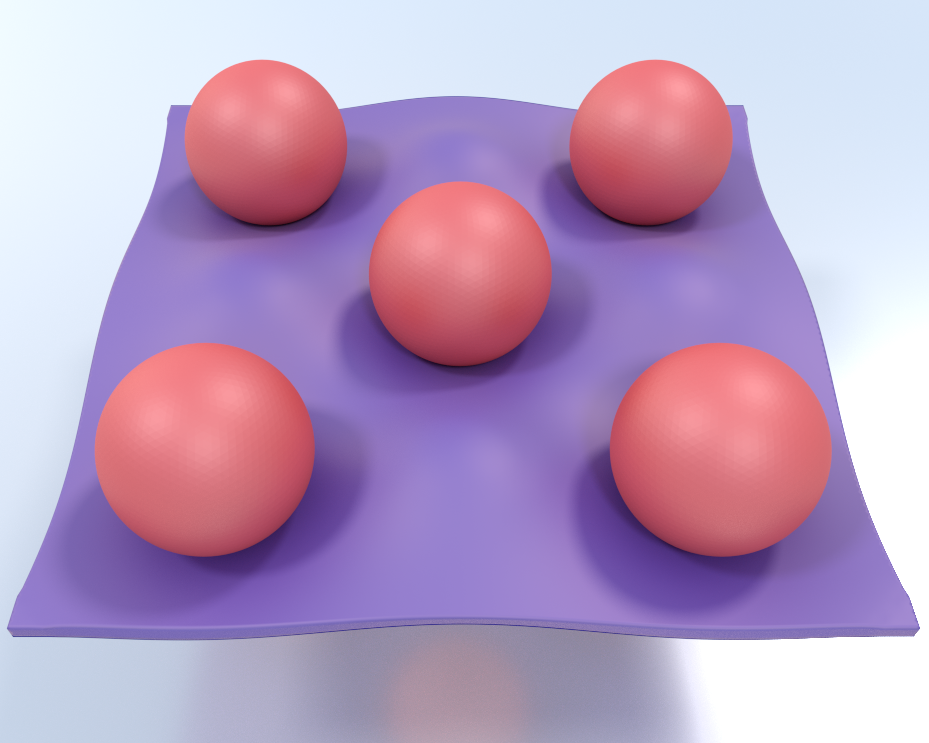
\includegraphics[width=.32\textwidth]{chapter_macroblocks/images/nineballs1.png} 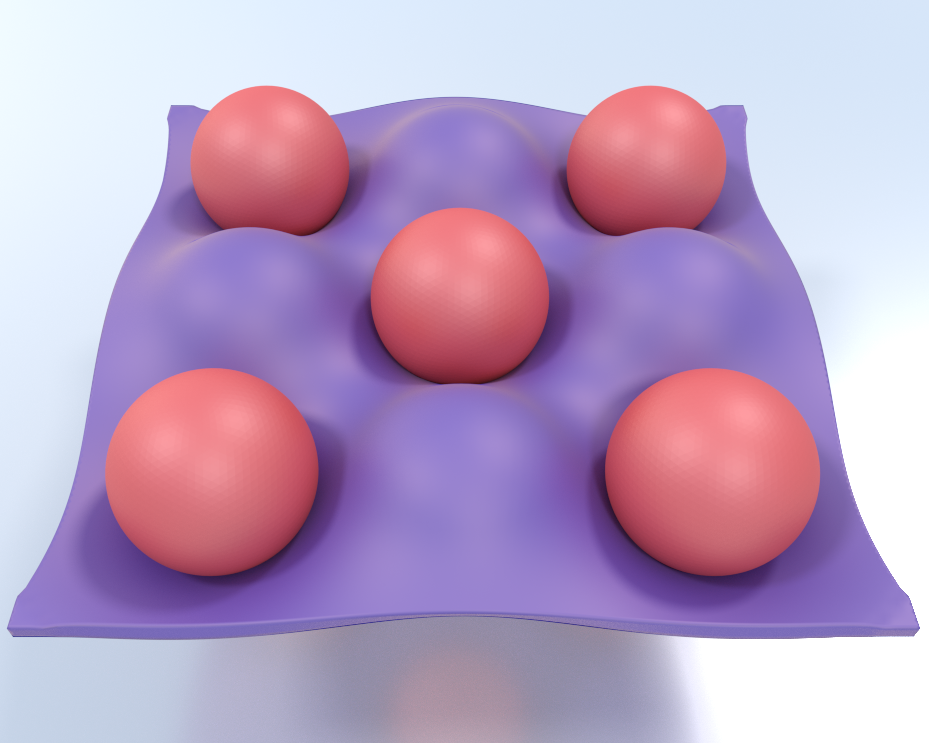
\includegraphics[width=.32\textwidth]{chapter_macroblocks/images/nineballs2.png} 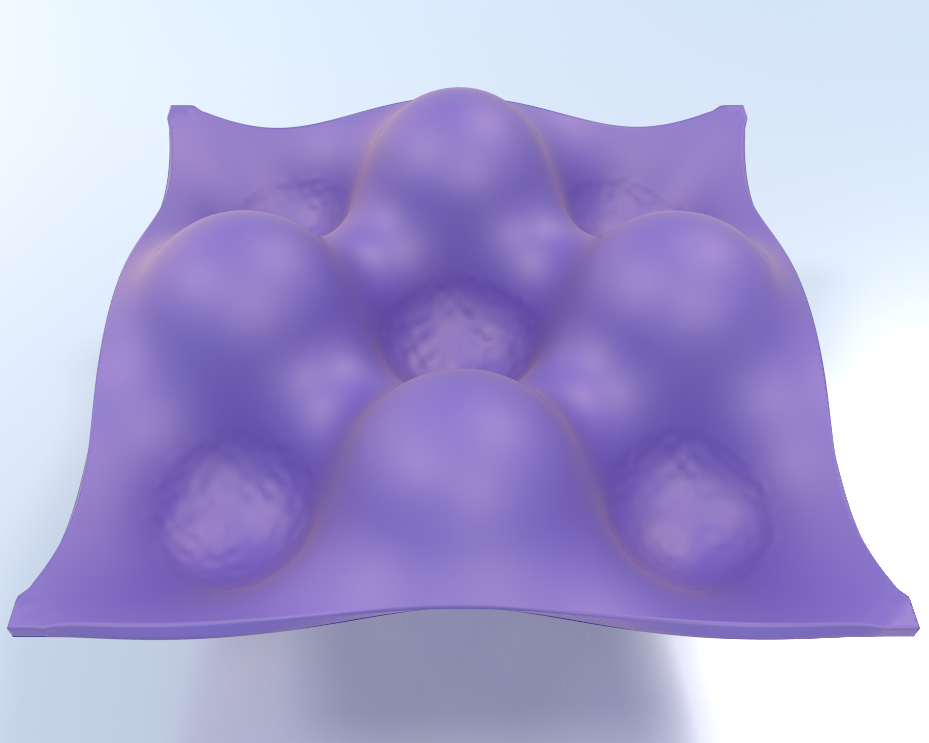
\includegraphics[width=.32\textwidth]{chapter_macroblocks/images/nineballs3.png} \end{center}
   \caption{Macroblock collision scenario unsuitable for multigrid
     techniques}{An array of 9 kinematic spheres, arranged in an
     alternating pattern across a thin volumetric sheet, are pressed
     against it. The limited thickness of this model would hinder
     applicability of stock geometric multigrid, in the absence of
     nonstandard coarsening strategies.}
    \label{fig:macroblocks:nineballs-example} \end{figure*}

\subsection{Vectorization}
\label{sec:macroblocks:vectorization}

\begin{figure*}[t!] \begin{center} 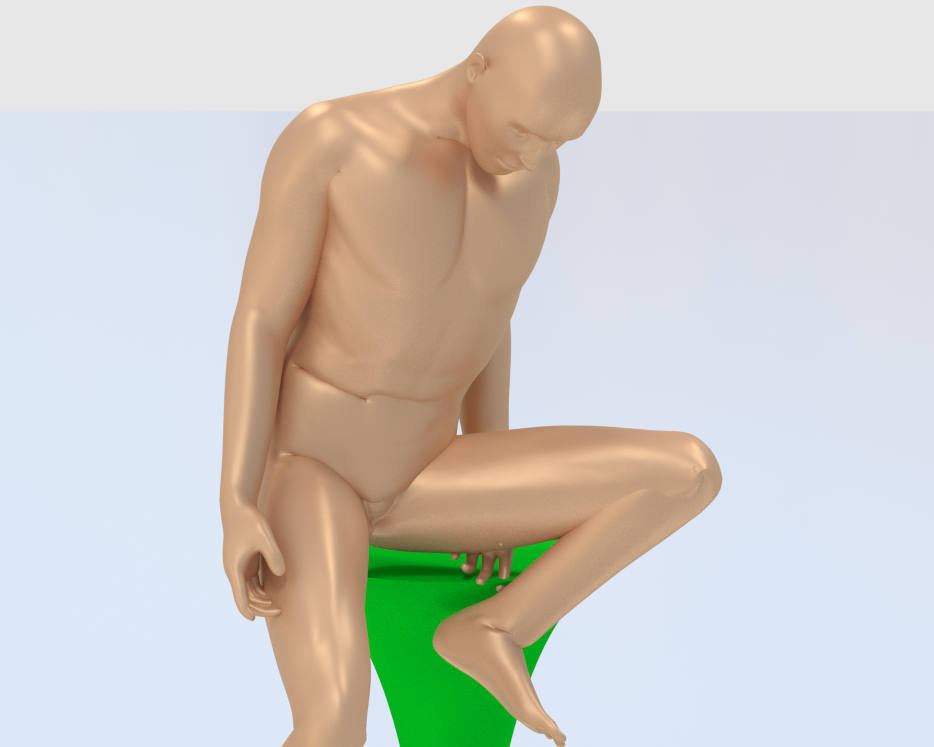
\includegraphics[width=.31\textwidth]{chapter_macroblocks/images/skinning2_skin.png} 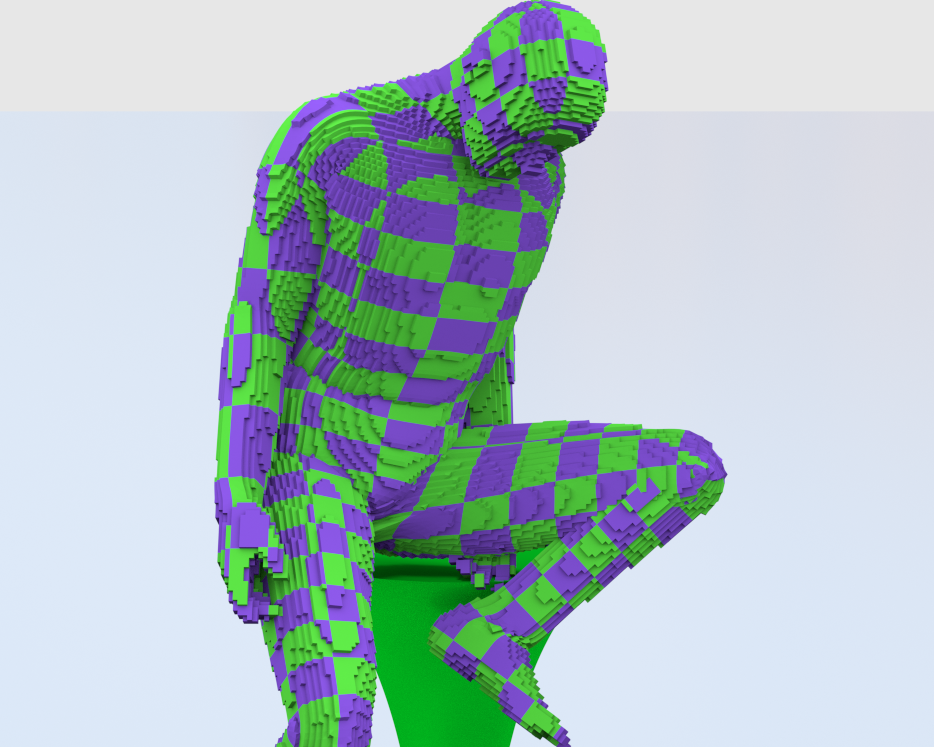
\includegraphics[width=.31\textwidth]{chapter_macroblocks/images/skinning2_macroblocks.png} 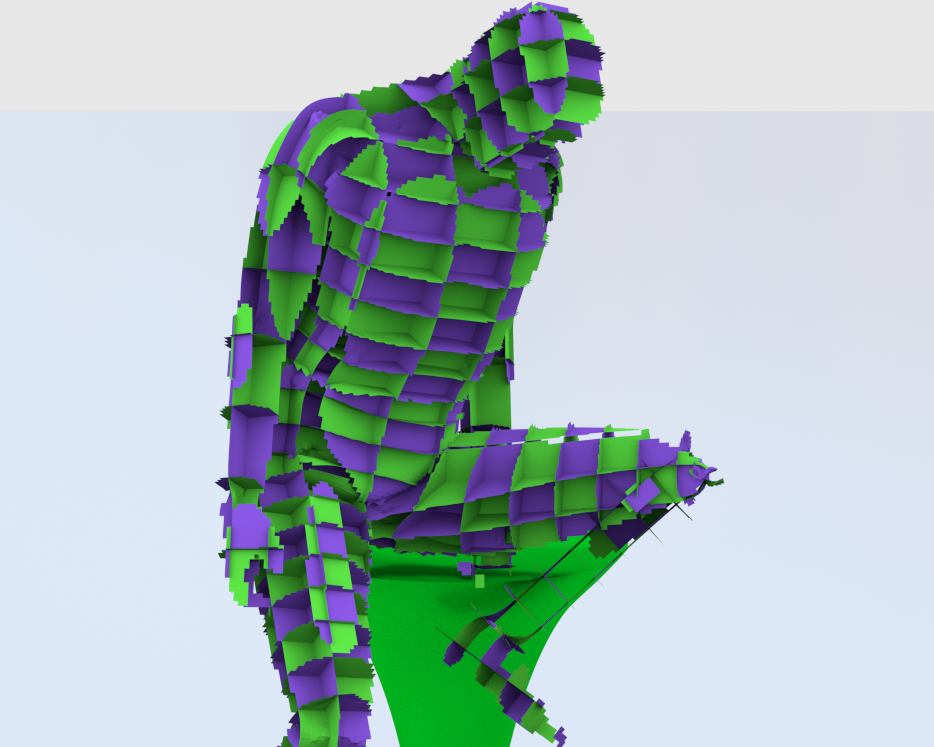
\includegraphics[width=.31\textwidth]
    {chapter_macroblocks/images/skinning2_interface.png} \end{center}
  \caption{Skinning simulation example with
    spring-attached bones}{An additional demonstration of a skinning
    simulation, driven by kinematic bones attached to the flesh via
    spring constraints.}
  \label{fig:macroblocks:skinning2-example} \end{figure*}

The sparse matrix data used in our method, as seen in figure
\ref{fig:macroblocks:sparsity2}, is characterized by extensive regular and
repetitive sparsity patterns that can facilitate computation using
SIMD instructions. We have used color coding to indicate data used
within a level of our hierarchical solution scheme, and to highlight
such patterns of regularity. Those include the sixteen sparse Cholesky
factors corresponding to the interiors of the $3\times 3\times 3$
subdomains (colored as dark blue blocks, along the top-leftmost part
of the matrix diagonal), the dense Cholesky factors of Schur
complements at deeper levels (eight magenta, four green, two orange,
and one cyan dense block, spanning the rest of the block-diagonal
region of the matrix), and sparse submatrices on the block
lower-triangular part of the matrix, corresponding to entries of the
original stiffness matrix that touch an interface layer at a given
level of the hierarchy and nodes on the two subregions that the
interface layer separates.

Opportunities for aggressive vectorization directly emerge from such
data regularities. For example, sparse forward and backward
substitution on all sixteen $3\times 3\times 3$ subdomains can be done
in tandem, with 16-way SIMD parallelism (e.g., using two 8-wide AVX
instructions). Repetitive sparsity patterns in the lower-triangular
part of the matrix of figure \ref{fig:macroblocks:sparsity2} are used in
vectorized matrix-vector multiplication operations. The \emph{dense}
nature of the blocks along the lower part of the block-diagonal allows
fine-grain vectorization via standard practices.  Furthermore, even
matrix operations that connect the $15\times 7\times 7$ interior node
set with the \emph{boundary} of the macroblock, as the multiplication
with matrices $\mathbf{K}_{\Gamma_i\Gamma_i}$,
$\mathbf{K}_{\Gamma_i\mathrm{I}_i}$ and
$\mathbf{K}_{\mathrm{I}_i\Gamma_i}$ defined in the beginning of this
section, can be vectorized by splitting up such matrices in parts that
correspond to the sixteen $3\times 3\times 3$ macroblocks at the
interior of the macroblock boundary. Ultimately, about 96\% of the
requisite computations can accommodate 16-wide SIMD parallelism, and
the majority of the remaining operations offer at least 8-wide SIMD
parallelism potential. We have extensively leveraged these
vectorization opportunities in our optimized implementation based on
AVX compiler intrinsics.

\section{Justification of macroblock size choice}
\label{sec:macroblocks:analysis}

Our choice for utilizing macroblocks of dimension $16\times 8\times 8$
was motivated by a number of factors. First, we wanted to provide the
opportunity for at least 16-way SIMD-based parallelism, which is a
future-safe choice given the upcoming availability of CPUs with the
AVX-512 instruction set. The working set size associated with
macroblocks of that size is conveniently approximately 800KB, which
allows the entire macroblock solver to fit entirely in cache, even if
all cores of a typical modern Xeon processor are processing
independent macroblocks, in parallel. Using an even larger macroblock
size would allow the dimensionality of the interface to be further
reduced, but the increment in the working set would be
disproportionately large, due to the size of the next-level interface
(would be $15\times 1\times 7$) which would, at that point, yield an
unattractively large dense Schur complement matrix for that interface
level.


%-------------------------------------------------------------------------

\section{Examples and performance evaluation}
\label{sec:macroblocks:examples}

We visually demonstrate the applicability of our solver to a number of
simulation scenarios including constraint-driven deformations,
skinning animations and elastic models colliding with kinematic rigid
objects.  We used a hexahedral finite element discretization of
corotated linear elasticity, with the standard adjustments for robust
simulation in the presence of inverted elements
~\citep{IrvinTF:2004}. Given that our method uses a direct solver at the
macroblock level, we opted to integrate the strain energy using the
eight Gauss quadrature points for each hexahedron, as opposed to the
one-point quadrature scheme that is often used
~\citep{McAdaZSETTS:2011,PatteMS:2012}. This more accurate quadrature
scheme does not require explicit stabilization, and adds no extra
algorithmic effort in our solver other than a modest increase in the
matrix construction cost.

In figure \ref{fig:macroblocks:armadillo-example}, we demonstrate an armadillo
model being deformed as a result of specific lattice nodes animated as
kinematic Dirichlet boundary conditions. In order to incorporate
Dirichlet boundary conditions in the interior of a macroblock, we
replace the equation associated with any such node with an explicit
Dirichlet condition $\delta\mathbf{x}_i=\mathbf{0}$ (the value can be
set to zero without loss of generality, since equation
(\ref{eqn:macroblocks:quasistatic}) is solved for position corrections, which are
zero for constraint nodes that have been already moved to their target
locations). We restore symmetry of the overall matrix by zeroing out
entries involving the Dirichlet node in the stencil of the elasticity
operator of any neighboring node (again, a safe operation as the
Dirichlet value is zero for the correction
$\delta\mathbf{x}_i$). Similarly, any nodes in a macroblock that are
exterior to the simulated model are treated as zero-Dirichlet
conditions, to maintain a constant matrix structure for all
macroblocks.

In figures \ref{fig:macroblocks:face-smash-example} and
\ref{fig:macroblocks:nineballs-example}, we demonstrate the compatibility of our
method with penalty-based collisions with kinematic objects. We use an
implicit representation for the colliding bodies to enable fast
detection of collision events between such bodies and embedded
collision proxies on the surface of our model. When such an event
occurs, a zero rest length penalty spring constraint is instantiated
connecting the offending point on the embedded surface to the nearest
point on the surface of the collision
object. %Although we did not conduct a comparative evaluation, we expect that the thin nature of the models in both of these examples would have made the application of a stock geometric multigrid %solver significantly less trivial in this context.
Finally, figures \ref{fig:macroblocks:skinning-example} and
\ref{fig:macroblocks:skinning2-example} show two examples of a human character
animated using embedded kinematic bone constraints. Skeletal motion
data was drawn from the CMU motion capture database
(\textsf{http://mocap.cs.cmu.edu}).

\renewcommand{\arraystretch}{1.2}
\setlength{\tabcolsep}{3pt}
\begin{table}[b!]
\centering
\caption{Performance results for the macroblock solver
  across several examples}{Runtime details on a 10-core Xeon E5-2687W CPU. The benchmark in the first column is repeated in the last two columns using stock CG, with one and eight quadrature points respectively. \textsf{Interface-Multiply} is the multiplication with the Schur complement.}
\label{tbl:performance_results}
\begin{tabular}{ p{4cm} | ccccc}
    \hline
                        & Human   & Armadillo & Human   & Human   &  \\
    \hline
Solver                      & \parbox[t]{3cm}{\centering Macroblock} & \parbox[t]{3cm}{\centering Macroblock} & \parbox[t]{2.5cm}{\centering CG (1-QP)} & \parbox[t]{2.5cm}{\centering CG (8-QP)}& \\
Active Cells                & 286K & 24K    & 286K  & 286K  &  \\
Macroblocks                 & 642     & 95        & \textit{N/A}      & \textit{N/A}      &  \\
\parbox[t]{4cm}{Interface Multiply}          & \parbox[t]{3.5cm}{\centering 27.6 ms (17 GB/s)} & \parbox[t]{3.5cm}{\centering 4.36 ms (16 GB/s) }  & \textit{N/A} & \textit{N/A}      &  \\
CG Iteration                & 33.3 ms & 5.22 ms   & 18.8 ms & 88.3 ms &  \\
Factorization               & 291 ms  & 88.0 ms   & \textit{N/A} & \textit{N/A}      &  \\
\parbox[t]{2.5cm}{Newton \\ Iteration} &   &     &   &   &  \\
\parbox[t]{2.5cm}{\hspace{.3cm} 10 CG} & 791 ms  & 166 ms    & 269 ms  & 958 ms  &  \\
\parbox[t]{2.5cm}{\hspace{.3cm} 20 CG} & 1.29 s  & 244 ms    & 462 ms & 1.84 s  &  \\
\parbox[t]{2.5cm}{\hspace{.3cm} 50 CG\\ } & 2.79 s  & 479 ms    & 1.07s  & 4.47 s  &  \\
\hline
\end{tabular}
\end{table}

\subsection{Performance benchmarks - Comparison to CG}
\label{sec:macroblocks:cgcompare}

Table \ref{tbl:performance_results} provides runtime details for
individual solver components. The first two columns correspond to the
models of figures \ref{fig:macroblocks:skinning-example} and
\ref{fig:macroblocks:armadillo-example}, and have been processed with our proposed
macroblock solver. In addition, we repeat the skinning simulation of
figure \ref{fig:macroblocks:skinning-example} using this time a highly optimized
and parallelized matrix-free implementation of unpreconditioned
Conjugate Gradients, borrowed from the work of \citet{MitchCS:2015}. While using this matrix-free CG solver, we
consider two discretization alternatives: (a) a one-point quadrature
scheme, with explicit stabilization
~\citep{McAdaZSETTS:2011,PatteMS:2012}, listed in the third column and
(b) a more accurate 8-point quadrature scheme matching the one in our
macroblock solver (fourth column). As mentioned, the quadrature scheme
does not affect the solve times of our method, once the matrix has
been constructed; the construction cost is included in the Newton
iteration runtimes, and was less than 10\% of the overall runtime in
all our experiments. We observe that, in spite of the up-front
factorization cost that our method incurs, it typically stays within a
factor of 2-3x of the cost of the single quadrature point CG scheme,
for the same number of iterations. Further experiments have shown that
the effect of as few as ten iterations of our macroblock scheme is
commensurate with 5-10x more iterations of the stock CG method. Note
that if the more accurate quadrature scheme is employed, our method
outperforms the CG option even on a per-iteration basis.

\subsection{Additional solver comparisons} 

We report some additional comparisons with other established numerical
algorithms or software packages. All our comparisons are relative to
the skinning example in the first column of Table
\ref{tbl:performance_results}.

\noindent\textbf{Macroblock inversion via Cholesky/PARDISO} As an
alternative to our optimized macroblock solver of section
\ref{sec:macroblocks:local-solver}, one could choose to directly compute
\emph{and} apply a stock Cholesky factorization per macroblock. We
tested this using the PARDISO library, which yielded a factorization
cost of 748ms (ours: 291ms) and a solve time of 93ms via
forward/backward substitution (ours: 20.9ms; part of the
\textsf{Interface-Multiply} cost). Solve time savings are due to our
reduced memory demands. Faster factorization time is attributed to
intrinsic knowledge about the constant sparsity pattern of each block,
allowing us to optimally vectorize over multiple blocks without
duplicating the data that captures their sparsity patterns.

\noindent\textbf{Different solvers for Newton Step} Three options were
investigated \emph{(a) Full Cholesky} -- We experimented with using a
direct (complete) Cholesky solve at each Newton step, via PARDISO. The
resulting Newton iteration cost was 31.8s, more than three times the
cost our method would require for 250CG iterations (9.36s) and
near-perfect convergence. However, our method hardly needs that many
CG iterations to achieve excellent Newton convergence, and in the long
run easily outperformed full Cholesky by more than an order of
magnitude. \emph{(b) Incomplete Cholesky PCG} -- ICPCG performed very
well in our examples, often requiring half (or less) of our CG
iterations for comparable convergence. It is, however, in principle a
serial algorithm. Our adequately optimized (albeit serial)
implementation required 7.23s to factorize the preconditioner (ours:
291ms) and 422ms (ours: 33.3ms) for each CG iteration. \emph{(c) Block
  Jacobi PCG} -- A parallelism-friendly alternative to ICPCG was to
compute a Block Jacobi Preconditioner, with block sizes comparable to
our own macroblocks. Matrix entries that straddle blocks were
discarded, and a standard Cholesky factorization of the resulting
block-diagonal matrix computed via PARDISO. Convergence of this option
was generally comparable, and at times slightly better than our
solver. This parallel method required 1.24s for factorization (ours:
291ms) and yielded a CG iteration cost of 183ms (ours: 33.3ms). 

%%% Local Variables:
%%% mode: latex
%%% TeX-master: "../document"
%%% End:
